\documentclass[aps,pre,twocolumn,superscriptaddress,showpacs]{revtex4-1}
%
%==================================================================
% PREFACE
%==================================================================
%
% BibTeX
\bibliographystyle{apsrev}
\bibliographystyle{plain}
%
%Packages
\usepackage{natbib}
\usepackage[english]{babel}
\usepackage[dvips]{graphics}
\usepackage{graphicx,epsfig}
\usepackage{amsmath}
\usepackage{color}
\usepackage{float}
\usepackage{multirow}
\usepackage[normalem]{ulem}
\usepackage{booktabs}
\usepackage{amsfonts} 
\usepackage{multirow}
\usepackage{subcaption}

%\allowdisplaybreaks

\newcommand{\om}{\omega}
\newcommand{\omx}{\omega_1}
\newcommand{\omy}{\omega_2}
\newcommand{\En}{\mathcal{E}_n}

%Text commands
\newcommand{\CR}[1]{{\color{red}{#1}}}
\newcommand{\CB}[1]{{\color{blue}{#1}}}
\newcommand{\CG}[1]{{\color{green}{#1}}}
\newcommand{\no}[1]{{\sout{\color{red}{#1}}}}
\newcommand{\nob}[1]{{\sout{\color{blue}{#1}}}}

\begin{document}
\title{Theoretical calculations of the Inelastic Confinement-Induced Resonances and its asymmetric splitting of two ultracold atoms trapped in optical lattices}
%
\author{Tom\'as S\'anchez S\'anchez-Pastor}
\affiliation{Grupo de Sistemas Complejos,
Escuela T\'ecnica Superior de Ingenier\'ia Agron\'omica,
Alimentaria y de Biosistemas,
Universidad Polit\'ecnica de Madrid,
Avda. Puerta de Hierro 2-4, 28040 Madrid, Spain.}

\author{Fabio Revuelta}
\affiliation{Grupo de Sistemas Complejos,
Escuela T\'ecnica Superior de Ingenier\'ia Agron\'omica,
Alimentaria y de Biosistemas,
Universidad Polit\'ecnica de Madrid,
Avda. Puerta de Hierro 2-4, 28040 Madrid, Spain.}

\author{Alejandro Saenz}
\affiliation{AG Moderne Optik, 
Institut für Physik, 
Humboldt-Universität zu Berlin, 
Newtonstrasse 15, 12489 Berlin, Germany.}
%
%------------------------------------------------------------------------------------
\begin{abstract}
movidas varias del abstract movidas varias del abstract movidas varias del abstract movidas varias del abstract movidas varias del abstract movidas varias del abstract movidas varias del abstract movidas varias del abstract movidas varias del abstract movidas varias del abstract movidas varias del abstract movidas varias del abstract movidas varias del abstract movidas varias del abstract movidas varias del abstract movidas varias del abstract movidas varias del abstract movidas varias del abstract movidas varias del abstract movidas varias del abstract
\end{abstract}
%------------------------------------------------------------------------------------
%\pacs{05.45.-a, 33.20.Tp, 82.20.-w}

\maketitle

%------------------------------------------------------------------------------------
\section{Introduction}  \label{sec:intro}
Contar un poco de historia de la observación de este tipo de resonancias, por qué los sistemas ultrafríos están de moda (control) y resonancias de Feshbach (cambiar B es cambiar a). Acoplamiento CM-Rel como causante de los cruces evitados, transiciones no adiabáticas y relacionarlo con el teorema adiabático.
%------------------------------------------------------------------------------------
\section{Two-atom numerical simulations}  \label{sec:system}
\subsection{Hamiltonian}
El Hamiltoniano, la solución teórica en forma integral de $a(E)$, términos del potencial del rm, CM y rm-CM. \cite{PhysRevLett.104.153202}

\subsection{Ab Initio calculations}
%------------------------------------------------------------------------------------
\section{Inelastic CIR}  \label{sec:theory}
Introducción contando en profundidad el origen de las ICIR, la aproximación de Simón y lo de la C.

\subsection{3-D}
jjejejeje

	\begin{figure}[H]
   	 \centering
    	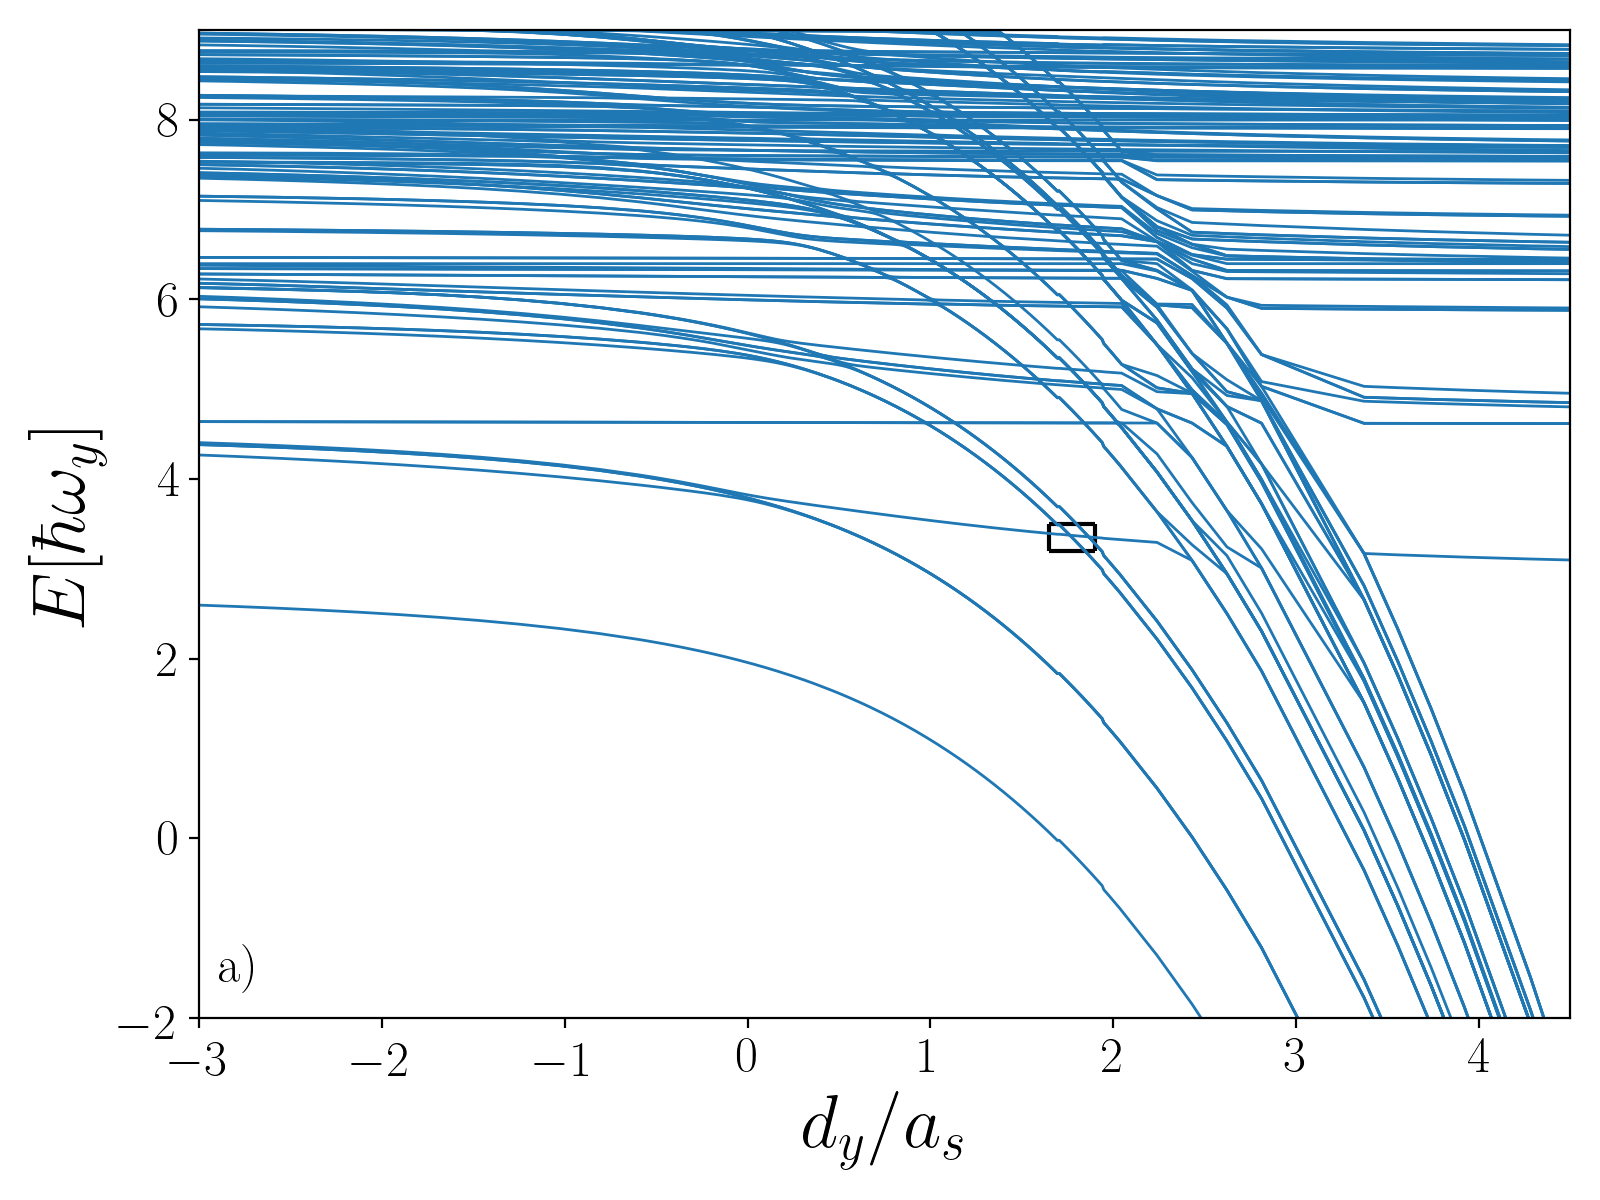
\includegraphics[scale=0.30]{/Users/tomy/PhD/Ultracold_Atoms_src/Analysis/q3d/Results/Figures/Ix4993_Iy4993_Iz4993_Easc_solid.png}
    	\caption{Adiabatic Spectrum of the full coupled Hamiltonian for $^7$Li atoms confined in an isotropic sextic trapping potential with $V_x = V_y = V_z = 35.9E_r$, $\eta_x = \eta_y = 1$ and $\lambda=1000$ nm. All states bending down to $-\infty$ are molecular states originating from the REL bound state $\psi^{(b)}$ with different CM excitations, whereas the states remaining constant are trap states of different REL excitations $\psi^{1}$ and zero CM excitations.}
    	\label{fig:3D spectrum}
	\end{figure}
	
	\begin{figure}[H]
   	 \centering
    	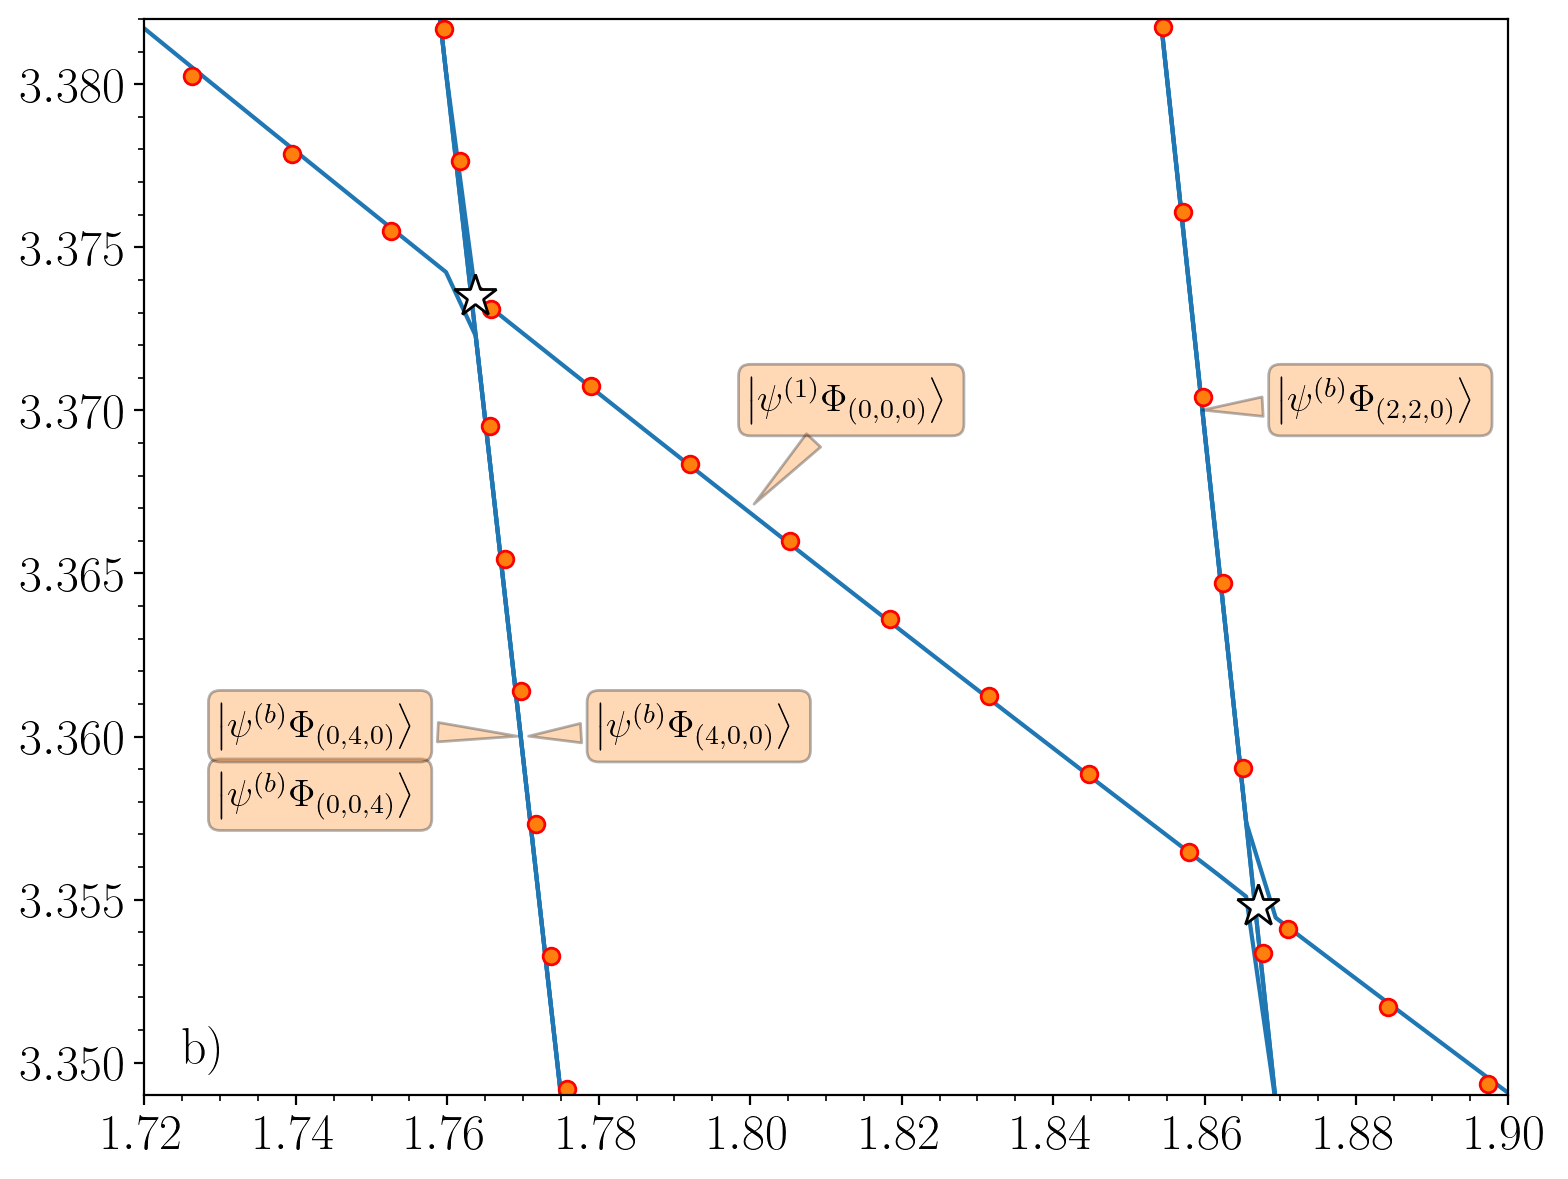
\includegraphics[scale=0.30]{/Users/tomy/PhD/Ultracold_Atoms_src/Analysis/q3d/Results/Figures/Ix4993_Iy4993_Iz4993_Easc_Interpolation_v2.png}
    	\caption{Zoom to the Inelastic CIR which arises from the avoided crossings between the first trap state and the transversally excited bound states. Diabatic states responsible of Inelastic CIR are drawn with red dashed lines and labeled by kets. For anisotropic transversal confinement the CIR splits in two due to the symmetry breaking.}
    	\label{fig:Isotropic Crossings}
	\end{figure}
	
	\begin{figure}[H]
	 \begin{subfigure}{0.5\textwidth}
	  \centering
	 \includegraphics[scale=0.30]{/Users/tomy/PhD/Ultracold_Atoms_src/Analysis/q3d/Results/Figures/ICIR_q3D.png}
	 \end{subfigure}
	 \vspace{10pt}
	 \begin{subfigure}{0.5\textwidth}
	   \centering
    	 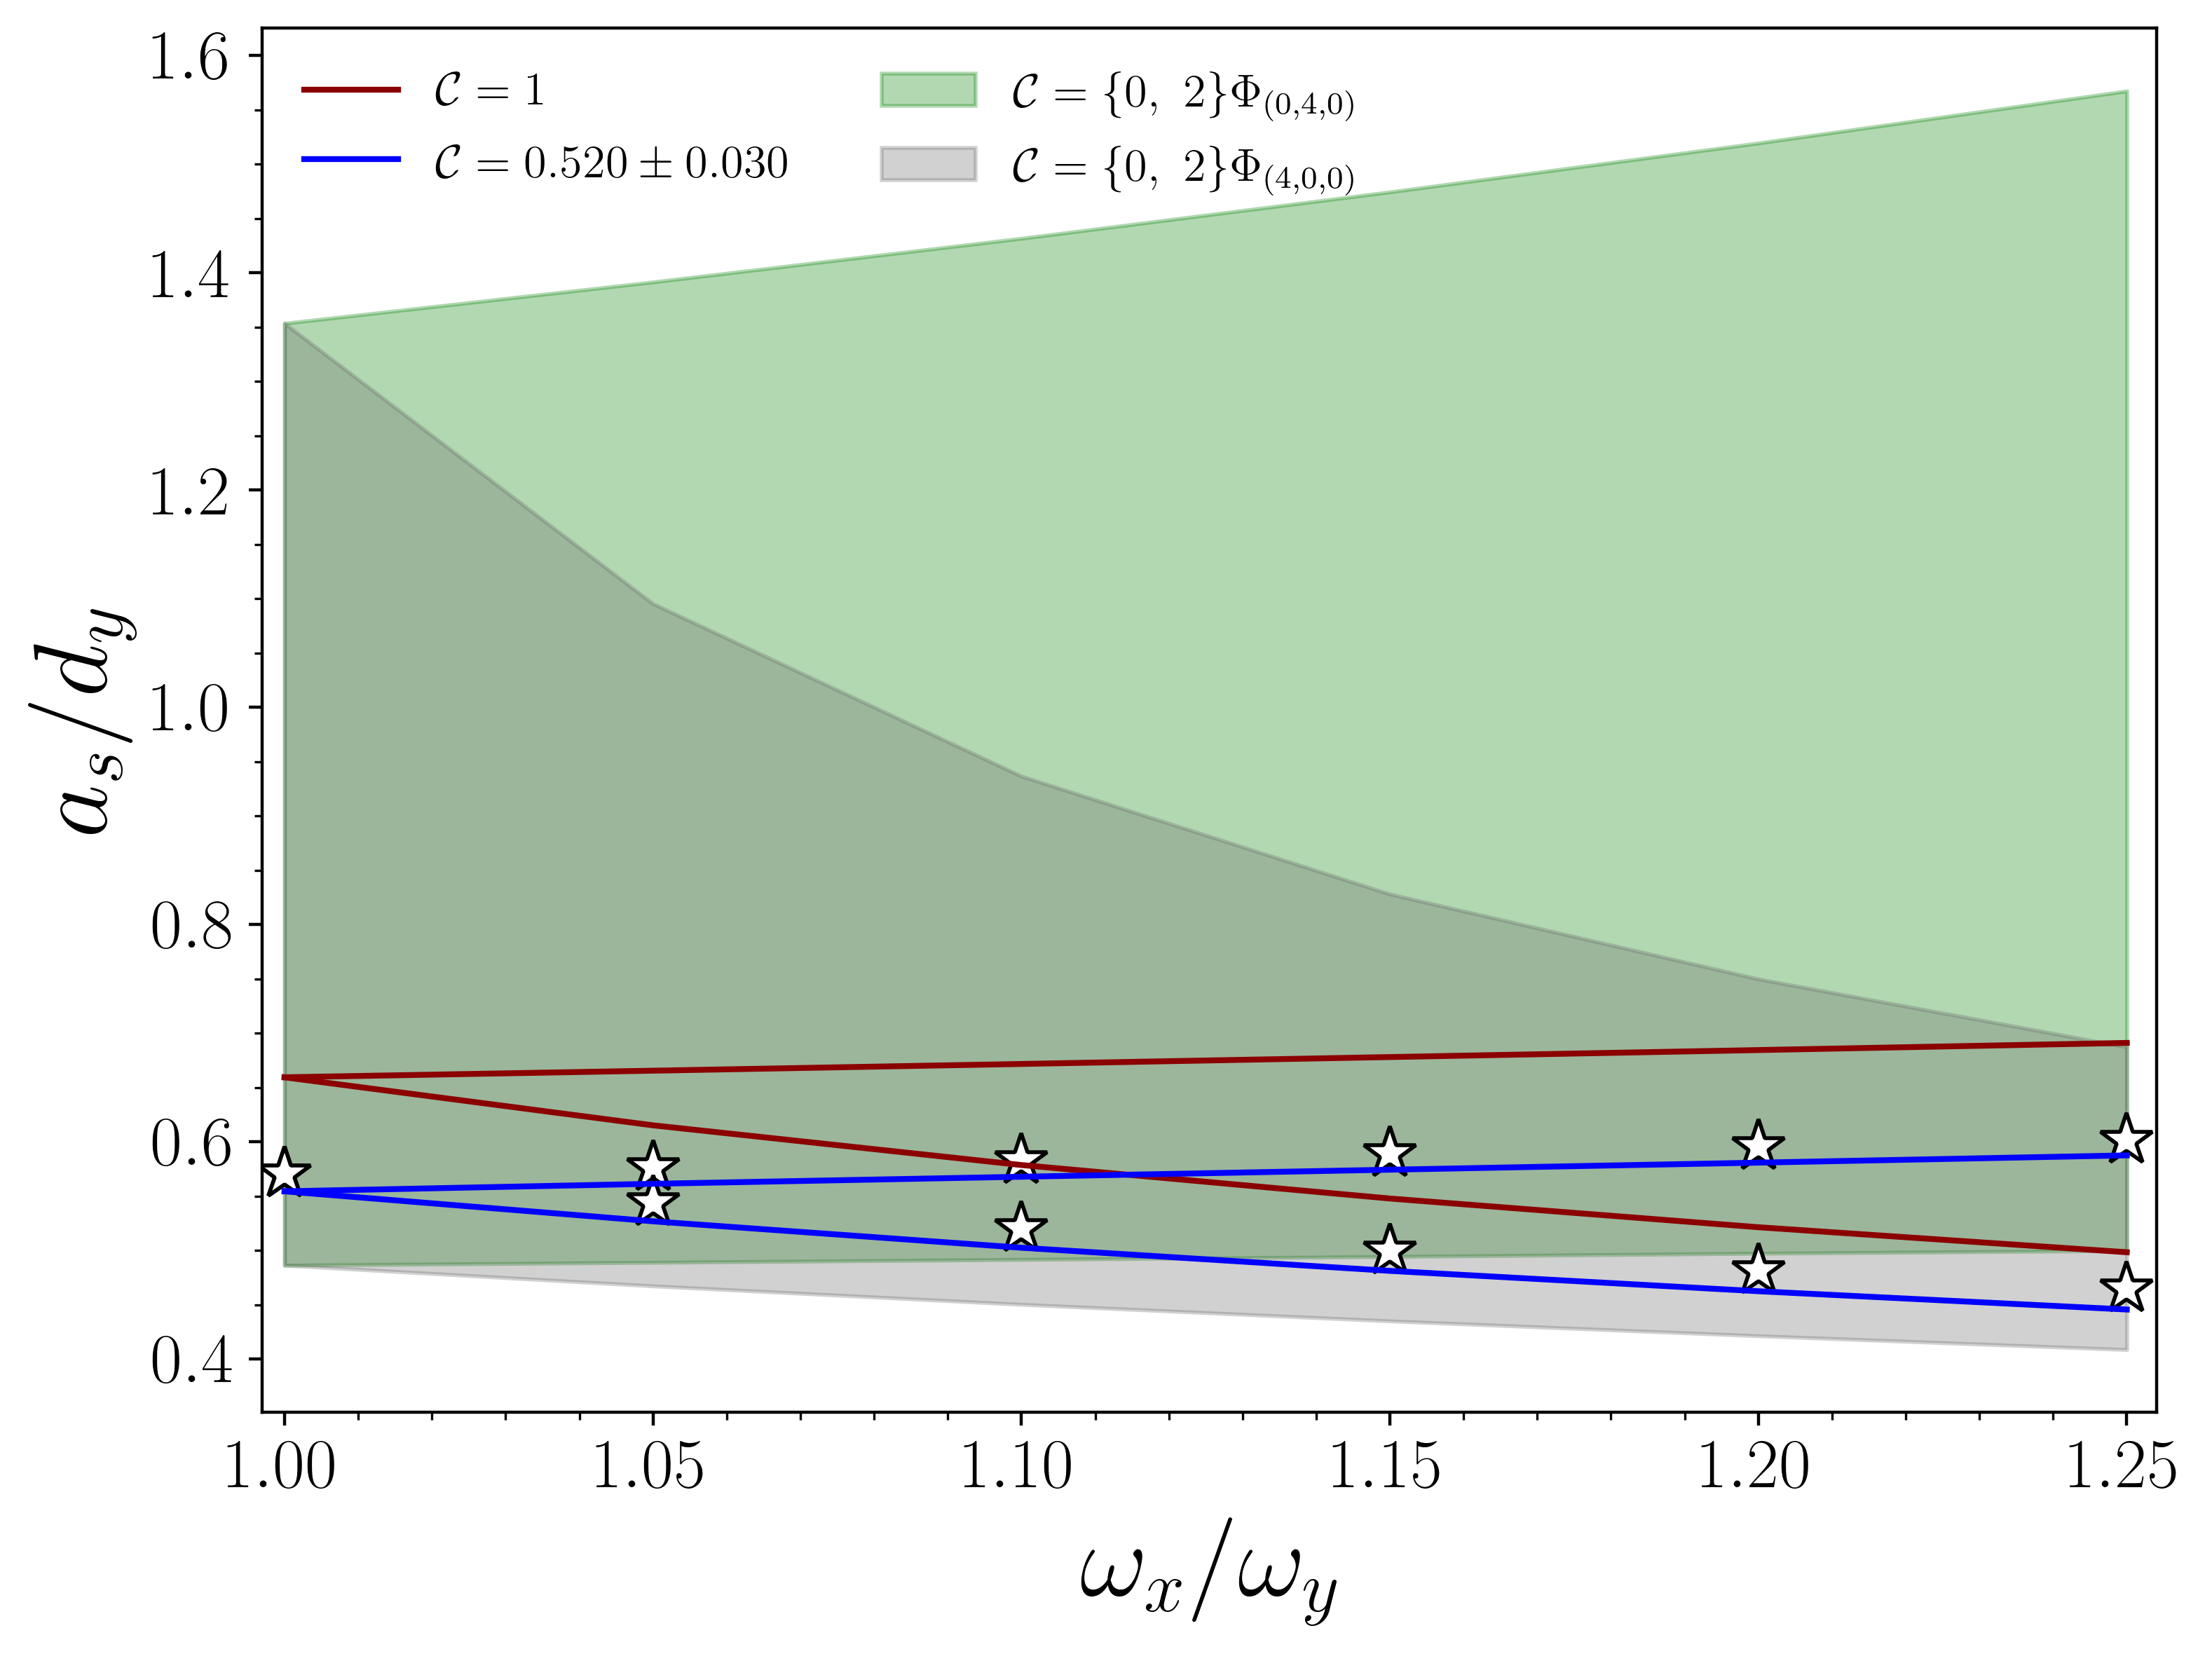
\includegraphics[scale=0.30]{/Users/tomy/PhD/Ultracold_Atoms_src/Analysis/q3d/Results/Figures/ICIR_q3D_Theory_band.png}
	 \end{subfigure}
    	\caption{Positions of the four excitations Inelastic CIR in terms of the characteristic transversal length for different values of transversal anisotropy in 3-D. Black stars are the ab initio calculations, blue dashed lines the exact theory computations with a constant $C=0.52\pm0.03$ and gray shadows the corresponding theory computations with both $C=2$ and $C=0$. }
    	\label{fig:q3d ICIR}
	\end{figure}
	
	%\begin{figure}[H]
%\centering
%\subfigure{\includegraphics[width=8cm, %height=6cm]{Union/dL(z)u.png}}\hspace{0.5mm}
%\subfigure{\includegraphics[width=8cm, height=6cm]{Golf/dL(z)g.png}}
%\label{Figura 1}
%\caption{M�dulo de distancias respecto al redshift para los datos de Union (izquierda) y Gold (derecha).}
%\end{figure}

%------------------------------------------------------------------------------------
\subsection{quasi 1-D}
\begin{figure}[H]
   	 \centering
    	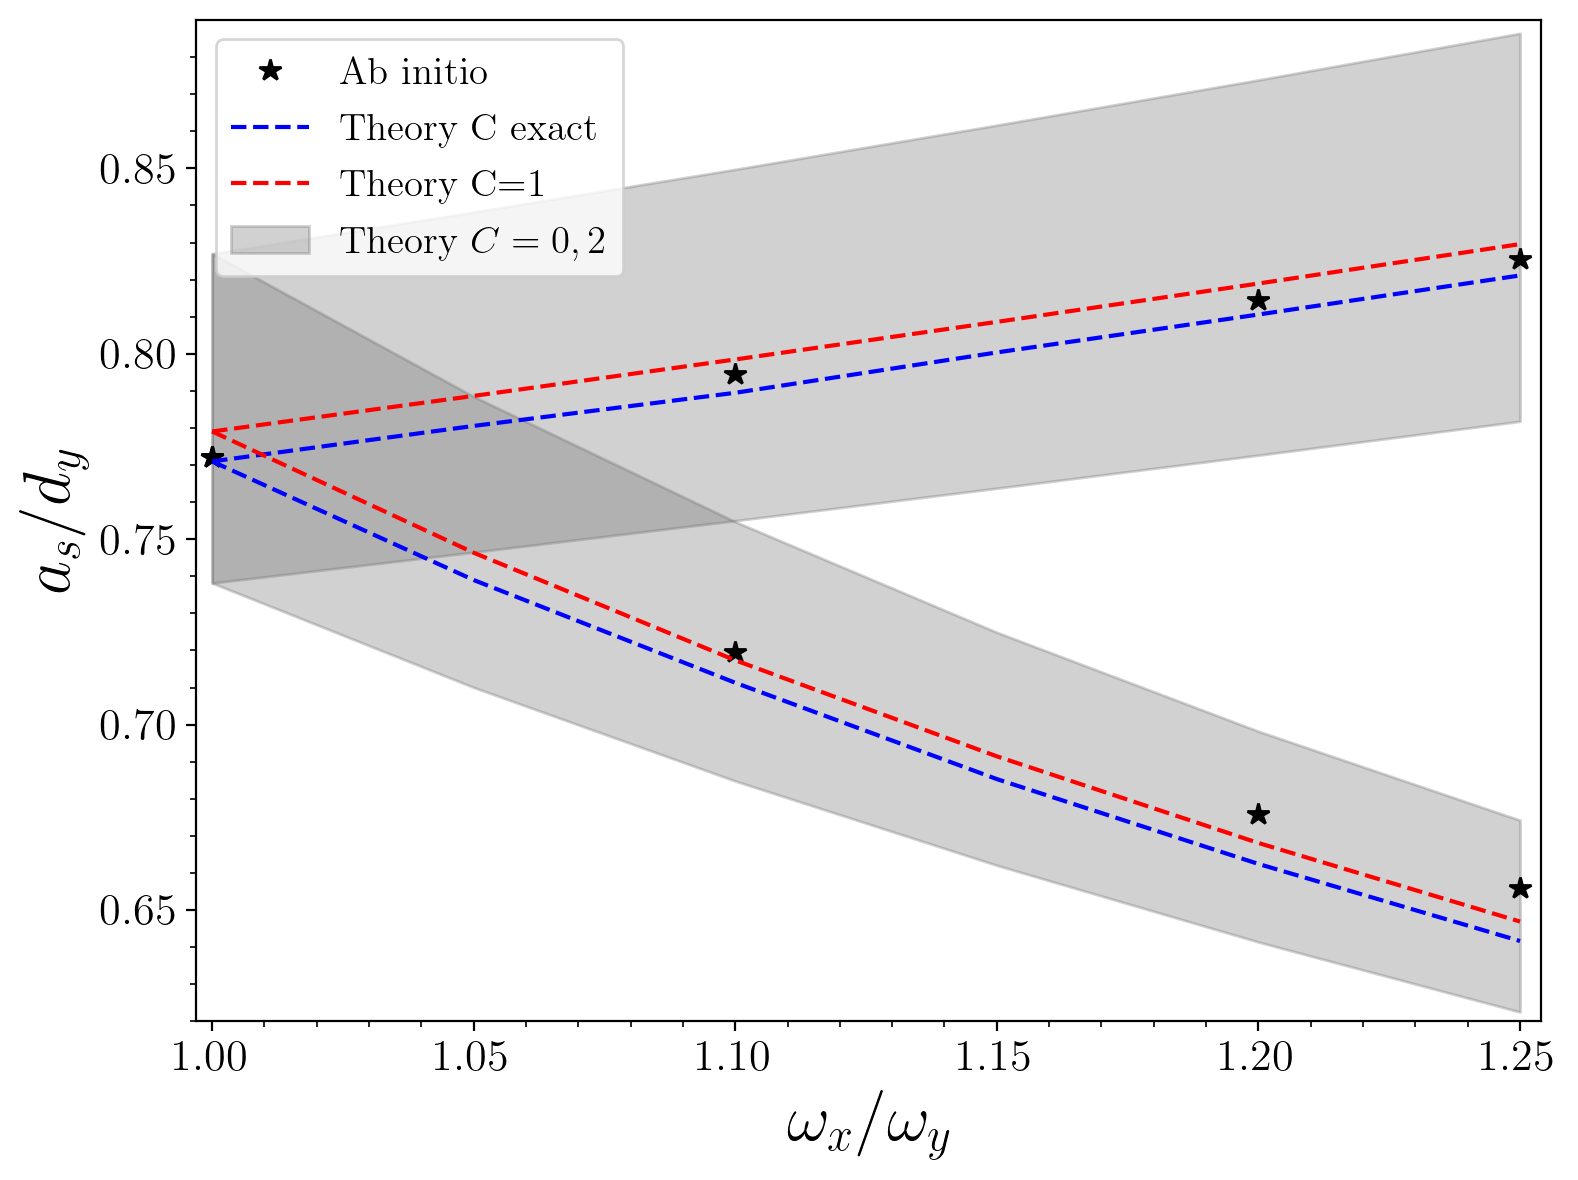
\includegraphics[scale=0.30]{/Users/tomy/PhD/Ultracold_Atoms_src/Analysis/q1d/Results/Figures/ICIR_q1D_Theory_band_coupling.png}
    	\caption{Positions of the two-excitations Inelastic CIR in terms of the characteristic transversal length for different values of transversal anisotropy in 3-D. Black stars are the ab initio calculations, blue dashed lines the exact theory computations with a constant $C=0.52\pm0.03$, red dashed lines $C=1$ and gray shadows the corresponding theory computations with both $C=2$ and $C=0$.}
    	\label{fig:q1D ICIR}
	\end{figure}

%------------------------------------------------------------------------------------
\section{Asymmetric splitting of the Inelastic CIR} \label{sec:perturbation}
Contar teoría de perturbaciones y lo que hizo Fabio

%------------------------------------------------------------------------------------
\section{Conclusions}
%------------------------------------------------------------------------------------
\section*{Anknowledgements}
%------------------------------------------------------------------------------------
\section*{References}
\bibliographystyle{unsrtnat}
\bibliography{q1d_q3d_perturbationCitation}

\newpage

\end{document}

















